\documentclass[12pt,oneside,notitlepage,abstracton,a4paper]{scrartcl}
\usepackage{epsfig,scrpage2,graphicx,subfig}
\usepackage{float}
\usepackage{hyperref}
\usepackage{listings}
\usepackage{csquotes}
\usepackage{color}
\usepackage{xcolor}

\definecolor{mygrey}{rgb}{0.97, 0.97, 0.98}
\lstset{
    backgroundcolor = \color{mygrey},
    language=C++,
    basicstyle=\ttfamily,
    breaklines=true,
    breakatwhitespace=true,
    inputencoding=utf8,
    extendedchars=true,
    keywordstyle=\color{blue}\ttfamily,
    numberstyle=\color{blue}\ttfamily,
    stringstyle=\color{red}\ttfamily,
    commentstyle=\color{green}\ttfamily,
    emph={void, int,char,double,float,unsigned,string,ifstream, std, TCT, :},
    emphstyle={\color{blue}},
    morecomment=[l][\color{magenta}]{\#}
    }
\lstset{literate={::}{}{0\discretionary{::}{}{::}}% line-break at ::
   {->}{}{0\discretionary{->}{}{->}}% line-break at ->
}

\setcounter{secnumdepth}{3}

\setlength{\parindent}{1.5em}
\usepackage{indentfirst}
\setlength{\parskip}{0ex plus0.5ex minus0ex}
\pagestyle{scrheadings}
\bibliographystyle{unsrt} 
\captionsetup[figure]{font=small,skip=0pt}

\renewcommand{\headfont}{\normalfont}

\cfoot{\pagemark}

% A picture on top of the titlepage
\subject{
\includegraphics[height=2cm]{pics/knu} 
\includegraphics[height=2cm]{pics/desy} 
\includegraphics[height=2cm]{pics/lpnhe}}

\title{\Large TCT-Analysis Framework Developers Guide} 
\author{ Mykyta Haranko \\ \footnotesize mykyta.haranko@gmail.com }

\date{\normalsize \today}

\begin{document}

\maketitle

\begin{abstract}

\noindent
This guide was written for users and developers of the TCT-Analysis framework to understand basic aspects of the program and to make them able to extend its functionality for further data analysis.
\end{abstract}

\newpage
\tableofcontents
\newpage 

\section{Introduction}\label{intro}

The Transient Current Technique (TCT) is widely used for studying the detector response after high irradiation fluences. The main idea is to use laser to produce charge carriers in the sensor, which is similar to the energy loss process of a minimum ionizing particle crossing the detector\cite{bib:haranko_desy}. Then waveforms are stored in a binary files and processed using different methods.
\\ \indent TCT-Analysis is a framework proposed by Hendrik Jansen and developed to make the data analysis process fast and unified for all the laboratories using this technique. The basic idea was to create one open source framework, to which people can easily add their analysis and share it with other people.
\\ \indent To implement new modules developer don't have to go deeply into the code and can go directly to the Sections~\ref{review:tct_module},~\ref{tutorial_impl}.

\section{Usage}\label{usage}

This section gives simple instructions on downloading, installation and usage of the framework, also gives a brief description of the configuration file.

\subsection{Downloading and Installation}\label{usage:installation}

There are two options available - console and graphical version of the framework. User can download pre-compiled Windows version or compile it from source.

\subsubsection{Pre-compiled version}

The pre-compiled version is distributed only for Windows, for the other operating systems it has to be compiled from source. TCT-Analysis requires ROOT 5.34.XX to be installed. Download needed version from \url{https://root.cern.ch/} and add it to the PATH environmental variable (usually offered by ROOT installer).
\\ \indent The next step is downloading the latest release of the framework from:
\begin{displayquote}
\url{https://github.com/DESY-FH-ELab/TCT-analysis/releases}
\end{displayquote}
Windows pre-compiled versions are stored in *.zip file. To install the program one needs to unzip the archive to the desired directory.
To start the program run \textbf{TCT-Analysis-QT.exe} in the \textbf{TCT-Analysis/bin} folder.
\\ \indent The last release was linked against ROOT 5.34.32. Tested on Windows 7, Windows 8.1 with ROOT 5.34.XX. Compiled using msvc2013 compiler.

\subsubsection{Compiling from source using CMake}

To compile the framework from source using CMake next prerequisites have to be satisfied:
\begin{itemize}
\item ROOT 5.X or 6.X has to be installed, ROOTSYS variable has to be defined.
\item CMake 2.6 or older has to be installed and added to the PATH variable.
\item (if GUI needed, \textbf{recommended}) Install Qt4 (Qt5 building with CMake not implemented for the moment).
\item (optional, for single waveforms acquisition) If LeCroy RAW data files converter needed - put the external LeCroyConverter lib to the \textit{external/LeCroyConverter/lib/libLeCroy.so}.
\end{itemize}

After satisfying dependencies, follow the next steps for both Windows and Linux operating systems:
\begin{enumerate}
\item Checkout the latest release of the program from the Github repository:
\begin{displayquote}
\url{https://github.com/DESY-FH-ELab/TCT-analysis/releases}
\end{displayquote}
Or go to the master branch to get the latest version in development
\begin{displayquote}
\url{https://github.com/DESY-FH-ELab/TCT-analysis}
\end{displayquote}
\item Go to the \textbf{TCT-Analysis/build} directory.
\item Run "\textbf{cmake $\langle$options$\rangle$ ..}" command with the next available options.
\begin{enumerate}
\item \textbf{-DWITH\_GUI=ON} -- compiles GUI version of the framework. Default -- OFF.
\item \textbf{-DWITH\_LECROY\_RAW=ON} -- links against LeCroyRAW Converter library. Default -- OFF.
\end{enumerate}
\item Run \textbf{make install}.
\item Go to the \textbf{TCT-Analysis/bin} directory.
\item Run \textbf{tct-analysis} or \textbf{tct-analysis.exe} executable.
\end{enumerate}

\subsubsection{Compiling from source using qmake}

To compile the framework from source using qmake next prerequisites have to be satisfied (compilation with GUI):
\begin{itemize}
\item For Linux: gcc 4.6 or later. For Windows: MSVC2015 or later.
\item ROOT 5.X or 6.X has to be installed.
\item Install Qt4 or Qt5.
\end{itemize}

After satisfying dependencies, follow next steps for both Windows and Linux operating systems:
\begin{enumerate}
\item Checkout the latest release of the program from the Github repository:
\begin{displayquote}
\url{https://github.com/DESY-FH-ELab/TCT-analysis/releases}
\end{displayquote}
Or go to the master branch to get the latest version in development
\begin{displayquote}
\url{https://github.com/DESY-FH-ELab/TCT-analysis}
\end{displayquote}
\item Open \textbf{TCT-Analysis.pro} file in \textbf{Qt Creator}.
\item Follow instructions to configure compilation of the program.
\item Change \textbf{TCT-Analysis.pro} file according to the location of ROOT libraries and include files.
\item Press \textbf{Ctrl+B} to build the program.
\item Repeat previous steps for \textbf{tbrowser.pro} file to compile \textbf{TBrowser}.
\item Both executables (\textbf{tct-analysis} and \textbf{tbrowser}) has to be placed in the \textbf{TCT-Analysis/bin} folder. 
\item Create \textbf{default.conf} file in \textbf{TCT-Analysis/bin} folder containing:
\begin{displayquote}
DefaultFile = ../testanalysis/lpnhe\_top.txt
\end{displayquote}
\item Run the program. Note: be sure that Qt libraries are present in the PATH variable (LD\_LIBRARY\_PATH for Linux) or in the execution folder, otherwise program may fail to start, the same is for ROOT libraries.
\end{enumerate}

\subsection{First Run}\label{usage:first_run}

The following folder structure is present in the base folder:
\begin{itemize}
\item \textbf{./bin} -- contains executables and linked libraries
\begin{itemize}
\item \textbf{./bin/default.conf} -- contains name of the config file loaded by default
\item \textbf{./bin/execution.log} -- log file of the program execution and data analysis
\item \textbf{./bin/tct-analysis.exe} -- execution of the program
\item \textbf{./bin/tbrowser.exe} -- TBrowser execution
\end{itemize}
\item \textbf{./results} -- here program stores output data by default
\item \textbf{./testdata} -- folder with test data, contains one data file with focus search at “lpnhe” folder
\item \textbf{./testanalysis} -- folder with sample program configuration files
\item \textbf{./testsensor} -- folder with sample sensor configuration files.
\end{itemize}
Depending on the selected options of compilation from Section~\ref{usage:installation} user can have either console or graphical version of the program.
\\ \indent In case of the console version of framework, file with configuration has to be specified: 
\begin{lstlisting}
./tct-analysis -af <path-to-configuration-file> 
\end{lstlisting}
for example 
\begin{lstlisting}
./tct-analysis -af ../testanalysis/lpnhe_top.txt
\end{lstlisting}

\indent In case of the graphical version, configuration file specified in \textbf{bin/default.conf} will be loaded by default. In Figure~\ref{fig:main} main window of the program is shown.

\begin{figure}[H]
    \centering
    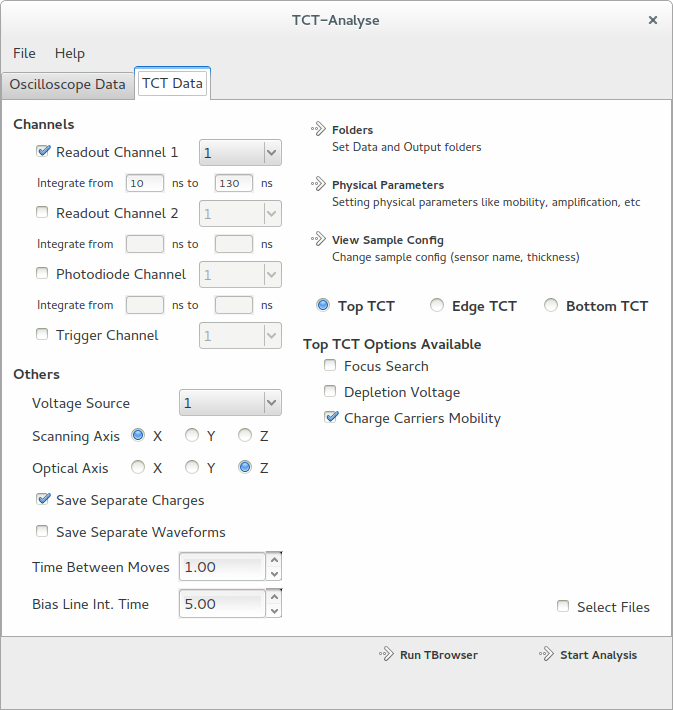
\includegraphics[width=8cm]{pics/main_window}
    \caption{Main window of the framework graphical version.}
    \label{fig:main}
\end{figure}

\indent To Open/Save new configuration file follow the corresponding file dialogue in the \textbf{File} menu at the top.
\\ \indent In Figure~\ref{fig:main_structure} structure of the main window explained with key control elements signed. 

\begin{figure}[h]
    \centering
    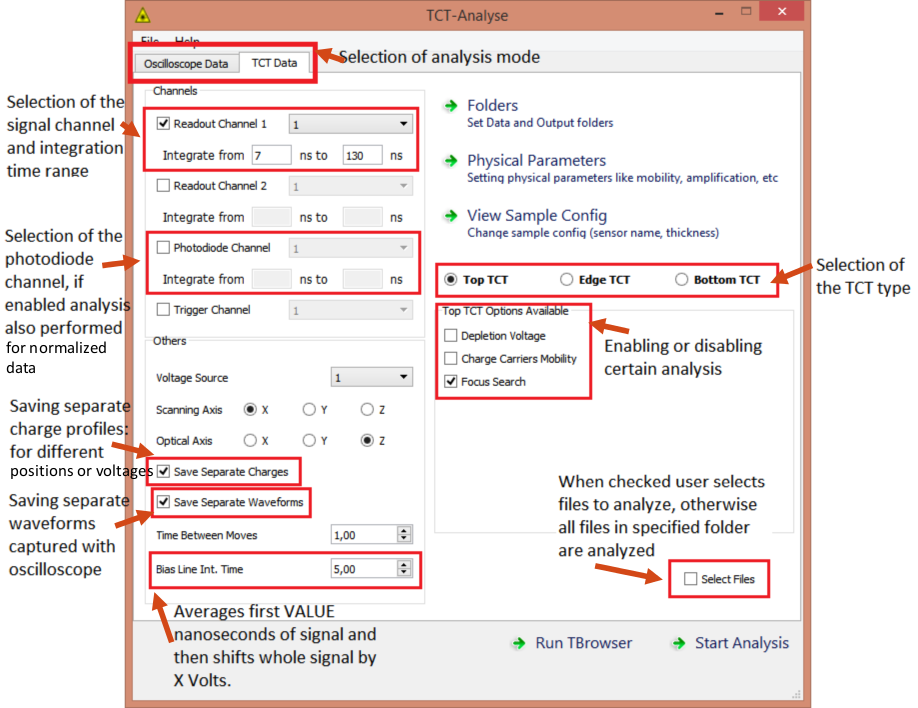
\includegraphics[width=18cm]{pics/main_structure}
    \caption{Structure of the main window.}
    \label{fig:main_structure}
\end{figure}

\begin{itemize}
\item To change data folder or output folder press \textbf{Folders} button.
\item \textbf{Physical Parameters} button is used to set physical quantities used for certain analysis.
\item \textbf{View Sample Config} used to change sensor name, thickness or general sensor configuration file.
\item \textbf{Run TBrowser} button is used to view output root files with analysed data.
\item To run analysis click \textbf{Start Analysis} button. If \textbf{Select Files} is checked, one need to select *.tct data file to analyse, otherwise all data files in the specified folder analysed.
\end{itemize}

\indent The program can operate in two modes: \textbf{TCT Data}, which analyses scans taken using PSTCT program from Particulars and \textbf{Oscilloscope Data}, which processes waveforms taken directly from the oscilloscope.
\\ \indent Normally for the graphical version user don't have to interact with the configuration *.txt file, but in case of the console version, configuration files are saved with comments, explaining all the parameters. Example of the configuration file is attached in Appendix~\ref{App:conf}.

\subsection{Sample Data File}\label{usage:sample}

Test analysis configuration file is present at the Github repository (\textbf{lpnhe\_top.txt}) and provided with the corresponding data file (\textbf{top\_focus\_precise.tct}), containing sample focusing scan data.
\\ \indent To run analysis in the console program version simply execute the next command:
\begin{lstlisting}
./tct-analysis -af ../testanalysis/lpnhe_top.txt
\end{lstlisting}
In the graphical version this configuration file is loaded by default. Click \textbf{Start Analysis} to run the program. Analysis Progress window will be displayed containing current progress on data analysis (Figure~\ref{fig:progress_analysis}). To view the results click \textbf{Run TBrowser} button.

\begin{figure}[h]
    \centering
    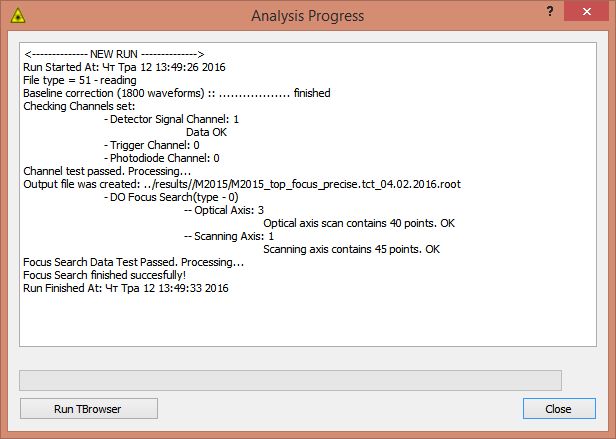
\includegraphics[width=12cm]{pics/progress}
    \caption{Analysis Progress window.}
    \label{fig:progress_analysis}
\end{figure}

By default results will be placed in
\begin{displayquote}
 \textbf{./results/M2015/M2015\_top\_focus\_precise.tct\_04.02.2016.root},
\end{displayquote}
this name consists of sample name, data file name and scanning date.
\\ Internal data structure is the next:
\begin{itemize}
\item \textbf{sample\_signals} -- contains sample signals from all the channels
\item \textbf{detector\_signals} -- contains all the signals from all the channels if \textit{Save Separate Waveforms} is checked
\item \textbf{“Scan Name”} -- contains data from certain analysis
\end{itemize}
For the \textbf{FocusSearch} scan the next graphs are available:
\begin{itemize}
\item \textbf{ChargeVsDistance} -- MultiGraph with all charge profiles on one graph
\item \textbf{./charges} folder -- contains waveforms for different positions along the optical axis
\item \textbf{FWHM} -- contains width of the falling edge from the charge profiles fit – this graph is the most important for the focus search
\item \textbf{MinCharge} -- can be used to cross check the FWHM fit. Contains minimal charge values when laser is lighting on the strip (usable when the strip width is comparable to the beam width)
\item \textbf{Missalignment} -- can be used to find the misalignment of the optical axis with respect to the scanning axis
\end{itemize}

To find additional information on the scan results interpretation see Section~\ref{modules} (partially, Section~\ref{modules:top:focus} for  Top TCT analysis output file interpretation).

\section{General Code Review}\label{review}

General program flow is the same for both graphical and console versions. In the following sections the console version of the program will be described by default, excepting remarks that will be made during the discussion.
\\ \indent The program can operate in two modes: \textbf{TCT Data} which analyses scans taken using PSTCT program from Particulars and \textbf{Oscilloscope Data} which processes waveforms taken directly from the oscilloscope.
\\ \indent After starting of the analysis process, the program follows next steps:
\begin{enumerate}
\item Reading of the configuration file with \lstinline$util$ class. It contains \lstinline$void parse(std::ifstream &cfgfile)$ method, which parses the configuration file and stores Keyword-Value pairs in \lstinline$std::map<std::string, std::string> _id_val$ map.
\item Parameters need to be converted to the corresponding type and stored in memory. Several classes of the same structure are used:
\begin{itemize}
\item \lstinline$mode_selector$ - is responsible for the program operation mode selection.
\item \lstinline$sample$ - is responsible for the sensor parameters storage.
\item \lstinline$tct_config$ - is responsible for the program operation in TCT Data mode.
\item \lstinline$analysis$ - stores configuration for the single waveforms from the oscilloscope analysis, also performs this analysis.
\end{itemize}
Each class mentioned above takes \lstinline$util$ class as the argument, then scans keywords for needed parameters and saves their values.
\item The analysis started in the selected mode. The programs scans data folder for needed file formats (*.tct files for TCT Data mode). 
\item \lstinline$Scanning$ class dynamic instance created.
\item Method \lstinline$bool Scanning::ReadTCT(char* filename, tct_config* config)$ called to analyse the data, passing file path and configuration class as the arguments. This method manages reading of the data file, runs the analysis and saves the result to the output file, for the details see Section~\ref{review:scanning}
\item Steps 4-5 are repeated for all the files found.
\end{enumerate} 

\subsection{Scanning Class}\label{review:scanning}

\lstinline$TCT:Scanning$ class manages reading of the data file, runs the analysis and saves the result to the output file. All the managing is done inside the \lstinline$bool Scanning::ReadTCT(...)$ method. In the source file one can see, that there are two different definitions of its header: in graphical version it sends the progress of the data analysis to the interface.
\\ \indent TCT data file is read using \lstinline$TCTReader$ class borrowed from Particulars and described in Section~\ref{review:data_reader}. \lstinline$ReadTCT$ method checks the file for presence of the data in specified channels using \lstinline$CheckData()$ method, creates *.root output file using \lstinline$CreateOutputFile()$ method, saves separate waveforms (if specified) and sample waveforms using \lstinline$Separate _and_Sample()$ method. After all the preparations it tries to run all the registered analysis modules checking if they are enabled and are of the same TCT type as selected. 

\subsection{TCT Data Reader}\label{review:data_reader}

\lstinline$TCTReader$ file contains two classes: \lstinline$TCTReader$ and \lstinline$TCTWaveform$. First one is responsible for reading of the data file, getting the histograms, etc. \lstinline$TCTWaveform$ is used to operate with multiple waveforms. Both classes were borrowed from \href{http://particulars.si}{Particulars}.
\\ \indent The most important methods of the \lstinline$TCTReader$ class are:
\begin{itemize}
\item \lstinline$TCTReader::TCTReader(char *FileNameInp, Float_t time0, Int_t Bin)$ -- constructor method, runs the read out of the data file
\item \lstinline$void  TCTReader::ReadWFsBin(Float_t time0)$ -- reads the waveforms
\item \lstinline$TH1F *TCTReader::GetHA(Int_t ch , Int_t x, Int_t y, Int_t z, Int_t nu1, Int_t nu2)$ -- returns the TH1F histogram for certain channel, position and voltage.
\item \lstinline$TCTWaveform *TCTReader::Projection(int ch, int dir,int x,int y,int z, int nu1, int nu2, int num)$ -- projects the data into the \lstinline$TCTWaveform$, which can be analysed later.
\item \lstinline$void TCTReader::CorrectBaseLine(Float_t xc)$ -- function corrects the baseline (DC offset) of all waveforms. It averages the signal in range (0,xc) and then shifts the signal by the mean value.
\item \lstinline$void TCTReader::PrintInfo()$ -- prints the file info.
\end{itemize}

\subsection{TCT Module Class}\label{review:tct_module}

\lstinline$TCTModule$ is the base class for module implementation. It contains basic functions for plotting,  integrating the histograms, checking the data, etc. It is run from \lstinline$Scanning$ class using the \lstinline$bool TCTModule::Do(TCTReader *in_stct, TFile *in_rootfile)$ method. To see the example of usage of the methods go to Sections~\ref{modules},~\ref{tutorial_impl}.
\\ \indent It consists of several base methods:
\begin{itemize}
\item \lstinline$TCTModule::TCTModule(tct_config* config1, const char* name, TCT_Type type, const char* title)$ -- module constructor method.
\begin{itemize}
\item \lstinline$tct_config* config1$ -- instance of the \lstinline$tct_config$ class
\item \lstinline$const char* name$ -- name of the class used internally, without spaces.
\item \lstinline$TCT_Type type$ -- type of the TCT measurement, can be: \_Top, \_Edge, \_Bottom.
\item \lstinline$const char* title$ -- title of the analysis, displayed everywhere.
\end{itemize}
\item \lstinline$bool TCTModule::Do(TCTReader *in_stct, TFile *in_rootfile)$ -- method called from outside to manage analysis process.
\item \lstinline$virtual bool TCTModule::CheckModuleData()$ -- \textbf{has to be re-implemented by developer}, checks the data is usable for the analysis. For example, focusing scan has to contain at least 10 points along the scanning axis to be able to fit the charge profile.
\item \lstinline$virtual bool TCTModule::Analysis()$ -- \textbf{has to be re-implemented by developer}, performs full analysis process.
\end{itemize}

There are several methods that have to be implemented when new \lstinline$TCTModule$ has additional analysis parameters, see Section~\ref{tutorial_impl} for additional information. These methods are used for the graphical version of the program and described below:
\begin{itemize}
\item \lstinline$virtual void PrintConfig(std::ofstream &conf_file)$ -- used to save parameter values to the file.
\item \lstinline$virtual void AddParameters(QVBoxLayout* layout)$ -- used to add these parameters to the interface. 
\item \lstinline$virtual void FillParameters()$ -- used to set the values of parameters to the interface widget.
\item \lstinline$virtual void ToVariables()$ -- used to read the values from the widget and save to variable.
\end{itemize}

To save time for implementing of new modules several methods were implemented and have to be used (when not specified argument supposed to be input):
\begin{itemize}
\item \lstinline$void SwitchAxis(Int_t sw, Int_t& nPoints, Float_t& step, Float_t& p0)$ -- used to briefly set the scanning axis.
\begin{itemize}
\item \lstinline$Int_t sw$ -- input, axis to set.
\item \lstinline$Int_t& nPoints$ -- output, variable containing the number of points.
\item \lstinline$Float_t& step$ -- output, the axis step.
\item \lstinline$Float_t& p0$ -- output, the starting point on axis.
\end{itemize}
\item \lstinline$void CalculateCharges(Int_t Channel, Int_t Ax, Int_t numAx,  Int_t scanning, Int_t numS, TGraph **charges, Float_t tstart, Float_t tfinish)$ -- calculating the charge profiles.
\begin{itemize}
\item \lstinline$Int_t Channel$ -- channel with signal.
\item \lstinline$Int_t Ax$ -- variable axis, optical axis for focusing, voltage for voltage scans.
\item \lstinline$Int_t numAx$ -- number of points for axis specified in previous step.
\item \lstinline$Int_t scanning$ -- the scanning axis id.
\item \lstinline$Int_t numS$ -- the scanning axis number of points.
\item \lstinline$TGraph **charges$ -- output, resulting charge profiles.
\item \lstinline$Float_t tstart$ -- integration time start, nanoseconds.
\item \lstinline$Float_t tfinish$ -- integration time start, nanoseconds.
\end{itemize}
\item \lstinline$TGraph** NormedCharge(TGraph** sensor, TGraph** photodiode, Int_t numP)$ -- normalizing charge profiles using photo diode signals.
\begin{itemize}
\item \lstinline$TGraph** sensor$ --  sensors charge profiles.
\item \lstinline$TGraph** photodiode$ -- charge profiles from photo diode.
\item \lstinline$Int_t numP$ -- number of profiles.
\end{itemize}
\item \lstinline$void FindEdges(TGraph* gr, Int_t numS, Float_t dx, Double_t &left_edge, Double_t &right_edge)$ -- searching for the sensor edges, useful in Edge TCT for defining sensor position.
\begin{itemize}
\item \lstinline$TGraph* gr$ -- charge profile used to find edges.
\item \lstinline$Int_t numS$ -- number of scanning points.
\item \lstinline$Float_t dx$ -- step.
\item \lstinline$Double_t &left_edge$ --  output, position of the left edge.
\item \lstinline$Double_t &right_edge$ -- output, position of the right edge.
\end{itemize}
\item \lstinline$void FindEdges(TGraph** gr, Int_t numP, Int_t numS, Float_t dx, Float_t* left_pos, Float_t* left_width, Float_t* right_pos, Float_t* right_width)$ -- the same as previous one, but for multiple charge profiles.
\item \lstinline$TGraph* GraphBuilder(Int_t N, Float_t *x, Float_t *y, const char *namex, const char *namey, const char *title)$ -- used to build graphs from x,y points, return TGraph pointer. 
\begin{itemize}
\item \lstinline$Int_t N$ --  number of points.
\item \lstinline$Float_t *x$ -- x-axis.
\item \lstinline$Float_t *y$ -- y-axis.
\item \lstinline$const char *namex$ -- title of the x-axis.
\item \lstinline$const char *namey$ -- title of the y-axis.
\item \lstinline$const char *title$ -- title of the graph.
\end{itemize}
\item \lstinline$void GraphBuilder(Int_t N, Float_t *x, Float_t *y, const char *namex, const char *namey, const char *title, const char *write_name)$ -- the same as previous one, but writes the graph directly to the output *.root file.
\begin{itemize}
\item \lstinline$const char *write_name$ --  name of the graph in the output file.
\end{itemize}
\item \lstinline$TGraph* GraphBuilder(Int_t N, Double_t *x, Double_t *y, const char *namex, const char *namey, const char *title)$ -- the same as the first GraphBuilder, but for Double\_t arrays.
\item \lstinline$void GraphBuilder(Int_t N, Double_t *x, Double_t *y, const char *namex, const char *namey, const char *title, const char *write_name)$ -- the same as the second GraphBuilder (with writing to the file), but for Double\_t arrays.
\item \lstinline$void GraphSeparate(Int_t N, TGraph **gr, const char *dir_name, const char *namex, const char *namey, const char *title, const char *name_0, Double_t *name_1)$ -- writes separate charge profiles to the file
\begin{itemize}
\item \lstinline$Int_t N$ --  number of charge profiles.
\item \lstinline$TGraph **gr$ -- charge profiles to write.
\item \lstinline$const char *dir_name$ -- directory to write.
\item \lstinline$const char *namex$ -- title of the x-axis.
\item \lstinline$const char *namey$ -- title of the y-axis.
\item \lstinline$const char *title$ -- title of the profiles.
\item \lstinline$const char *name_0$ -- name of the profile to write to the file, consists of string and number. This is string.
\item \lstinline$Double_t *name_1$ -- this is number.
\end{itemize}
\item \lstinline$void GraphSeparate(Int_t N, TGraph **gr, const char *dir_name, const char *namex, const char *namey, const char *title, const char *name_0, Float_t *name_1)$ -- the same as previous, but for Float\_t numbers to write (last argument).
\item \lstinline$void MultiGraphWriter(Int_t N, TGraph **gr, const char *namex, const char *namey, const char *title, const char *write_name)$ -- used to output the multi-graph with all the charge profiles.
\begin{itemize}
\item \lstinline$Int_t N$ --  number of charge profiles.
\item \lstinline$TGraph **gr$ -- charge profiles to write.
\item \lstinline$const char *namex$ -- title of the x-axis.
\item \lstinline$const char *namey$ -- title of the y-axis.
\item \lstinline$const char *title$ -- title of the graph.
\item \lstinline$const char *write_name$ -- name to write to the file.
\end{itemize}
\item \lstinline$void SetFitParameters(TF1* ff, Double_t p0, Double_t p1, Double_t p2, Double_t p3)$ -- simply sets the fit parameters values to the fit function, used to save space.
\begin{itemize}
\item \lstinline$TF1* ff$ --  fit function.
\item \lstinline$Double_t p0$ -- parameter 0.
\item \lstinline$Double_t p1$ -- parameter 1.
\item \lstinline$Double_t p2$ -- parameter 2.  
\item \lstinline$Double_t p3$ -- parameter 3.
\end{itemize}
\item \lstinline$Double_t GraphIntegral(TGraph *gr, Double_t x1, Double_t x2)$ -- integrates the graph in x1 to x2 range.
\item \lstinline$Double_t abs(Double_t x)$ -- return the absolute value of x.
\item \lstinline$void ChargeCorrelationHist(TGraph** sensor, TGraph** photodetector, Int_t numO)$ -- build a charge correlation histogram to check the correlation of sensor and diode signals.
\begin{itemize}
\item \lstinline$TGraph** sensor$ --  sensor charge profiles.
\item \lstinline$TGraph** photodetector$ -- photo detector charge profiles.
\item \lstinline$Int_t numO$ -- number of graphs.
\end{itemize}
\end{itemize}

To add the new analysis (module) to the program, one need to inherit it from the \lstinline$TCTModule$ class and place corresponding files to the \textbf{./src/modules} and \textbf{./include/modules} directories. The next is registering of the module, it has to be done in \textbf{./src/tct\_config.cc} file by calling RegisterModule method. For details, follow tutorial in Section~\ref{tutorial_impl}.

\section{Implemented Modules}\label{modules}
\subsection{Top TCT}\label{modules:top} 

\indent Top-TCT is defined by illuminating of the sensor top surface. Top-TCT is used to extract such quantities as the depletion voltage, velocity of the charge carriers, which is used for calculation of the mobilities of electrons and holes.

\subsubsection{Focus Search}\label{modules:top:focus}

\textbf{Idea}
\begin{figure}[h]
    \centering
    \subfloat[Scan along X axis.]{{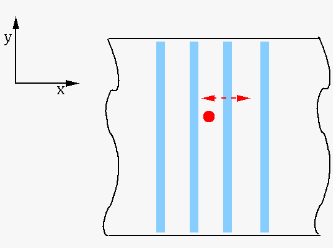
\includegraphics[width=6cm]{pics/top_focus_0} }}
    \qquad
    \subfloat[Changing of the beam spot size due to the different optical distances.]{{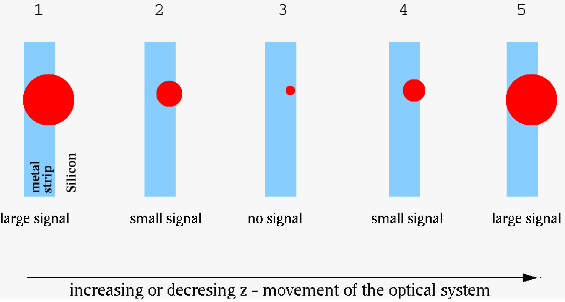
\includegraphics[width=10cm]{pics/top_focus_1} }}
    \caption{Schematic representation of the focus search method for a strip detector.\cite{bib:focus}}
    \label{fig:top_focus}
\end{figure} 

To find the focus for a strip sensor one need to follow instructions proposed in Ref.\cite{bib:focus}. The basic idea is shown in Figure~\ref{fig:top_focus}(a): when moving the beam spot along the X axis, less charge will be observed at the strip region - part of light will be reflected from the strip. Then, by changing the optical distance, the size of the beam spot can be changed (Figure~\ref{fig:top_focus}(b)). In Figure~\ref{fig:top_focus_1} the curves for focused and un-focused beam are shown. If the beam is out of focus, charge measured using the sensor, starts to increase slowly when scanning along the X-axis. This curve could be fitted using the error function, and the FWHM value can be extracted from the fit. When the beam spot gets smaller, the same happens to the FWHM value.  

\begin{figure}[h]
    \centering
    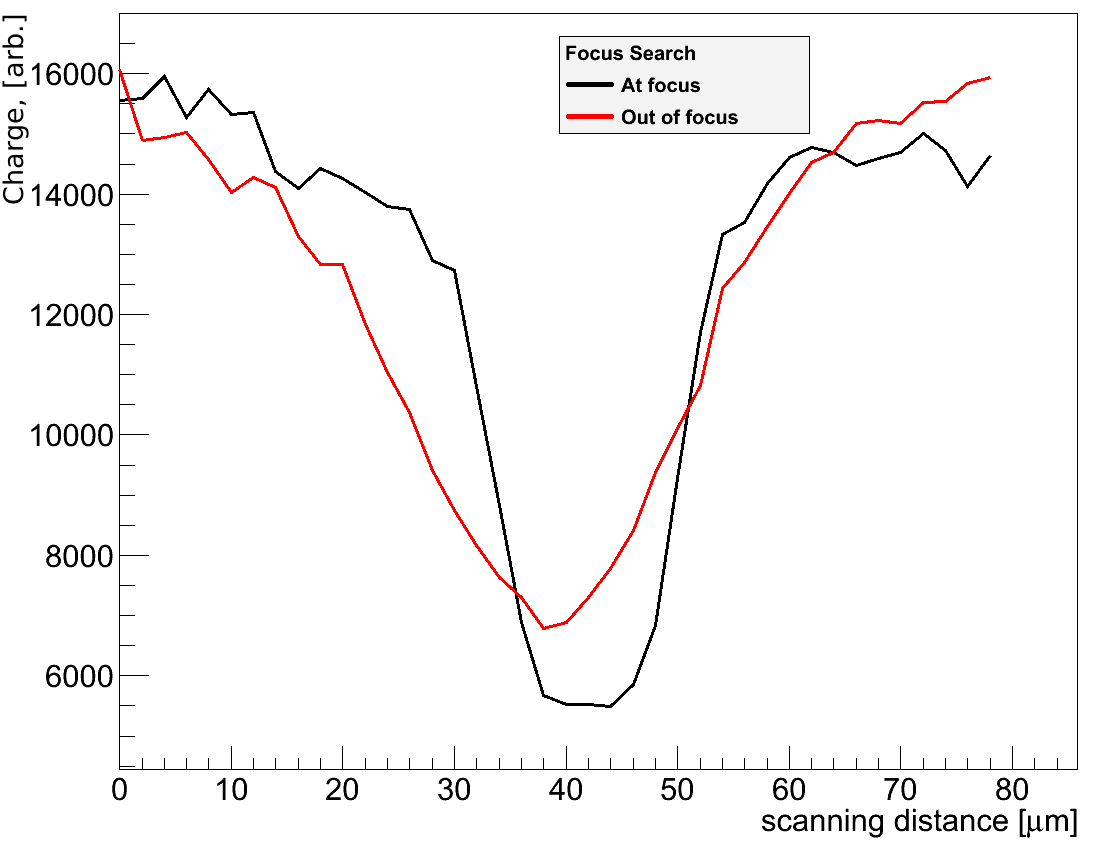
\includegraphics[width=8cm]{pics/top_focus}
    \caption{Scans for focused and un-focused beam, Top-TCT.}
    \label{fig:top_focus_1}
\end{figure} 

The FWHM is plotted for different optical distances and fitted with the second-order polynomial, see Figure~\ref{fig:top_focus_2}. The position with the smallest value of the FWHM is defined to be a focus position.

\begin{figure}[H]
    \centering
    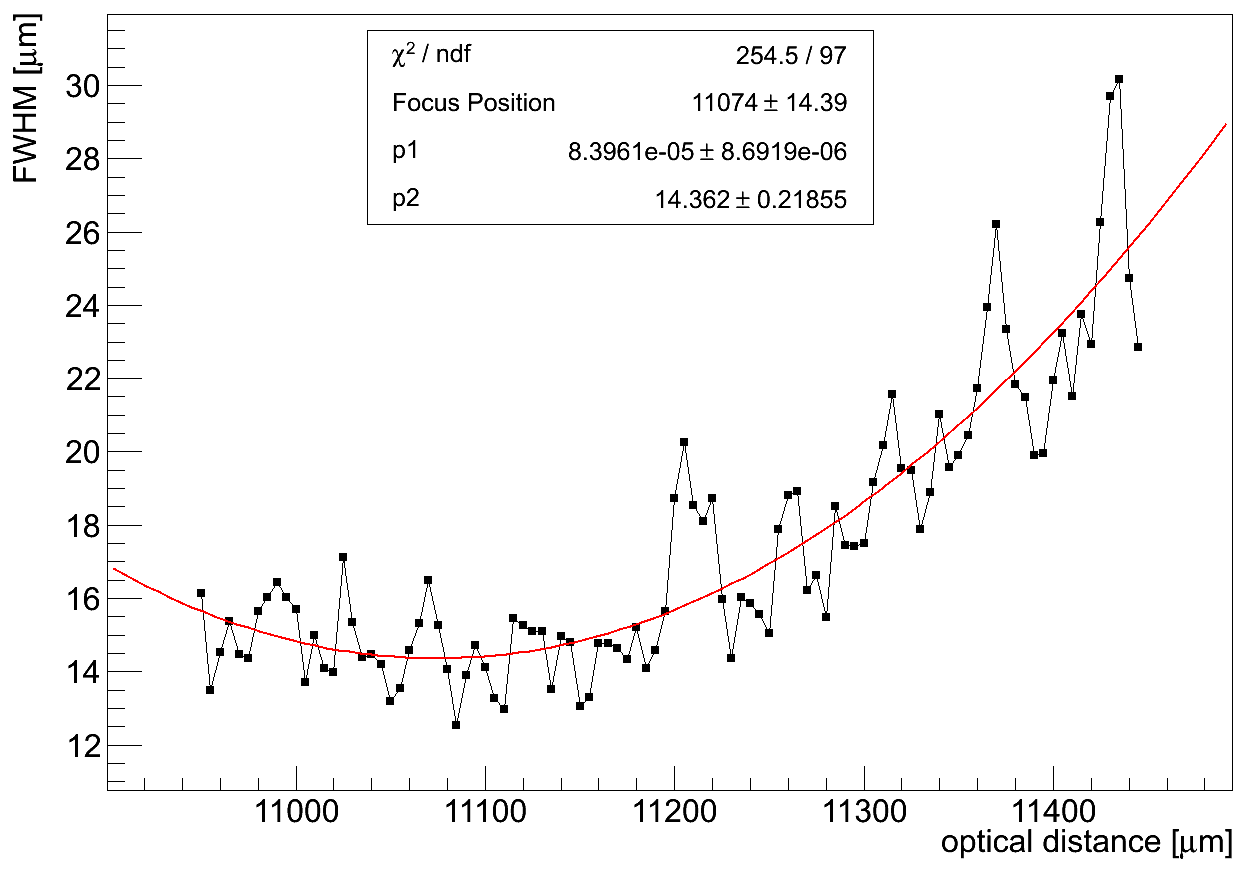
\includegraphics[width=11cm]{pics/top_focus_2}
    \caption{FWHM values for different optical positions, Top-TCT.}
    \label{fig:top_focus_2}
\end{figure}

\textbf{Realization}

\indent Top TCT Focus Search is realized in the \lstinline$ModuleTopFocus$ class inherited from the \lstinline$TCTModule$ class. The \lstinline$CheckModuleData()$ class method checks that scanning axis contains more than 10 scan points to be sure that charge profiles can be fitted. The \lstinline$Analysis()$ class method performs charge profiles building and fitting.

\subsubsection{Depletion Voltage}\label{modules:top:depl}

\textbf{Idea}

\indent To find the depletion voltage, the charge collected at certain position between strips for the different bias voltages has to be integrated. After reaching the depletion voltage charge stops to increase and becomes constant. Plotting the charge with square root of voltage, the dependency can be obtained, which has to be fitted with two lines - one fits the rising part, second one - the constant part, when all charge is collected ( detector is fully depleted ). The intersection of these curves gives the value of the full depletion voltage. For the sample sensor from Particulars Figure~\ref{fig:top_depl} shows the depletion voltage value of 33.6 V.

\begin{figure}[H]
    \centering
    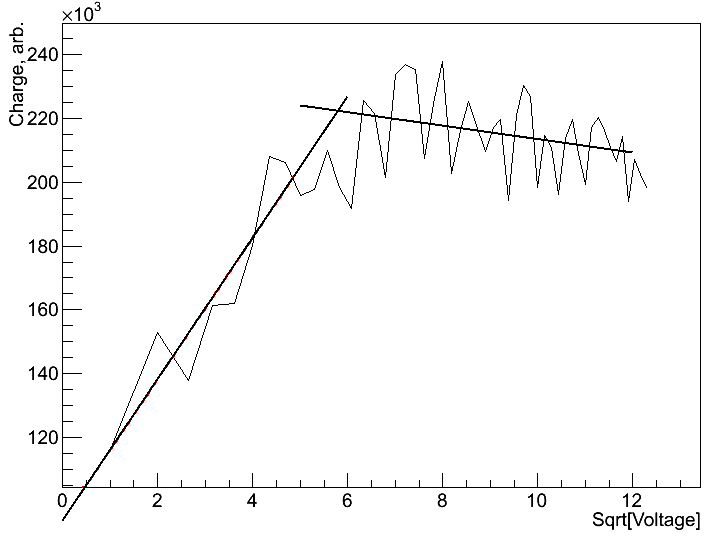
\includegraphics[width=9cm]{pics/top_depl}
    \caption{Depletion voltage search, Top TCT.}
    \label{fig:top_depl}
\end{figure}

\textbf{Realization}

\indent Top TCT Depletion Voltage search is realized in the \lstinline$ModuleTopDepletion$ class inherited from the \lstinline$TCTModule$ class. The \lstinline$CheckModuleData()$ class method checks that voltage scan contains at least 7 scan points to be sure that charge dependency vs. voltage can be fitted. The \lstinline$Analysis()$ class method performs charge dependency building and fitting.

\subsubsection{Mobility}\label{modules:top:mobility}

\textbf{Idea}

\indent The TCT is used to calculate the charge carrier mobility. The 80\% of the red light is absorbed after 5 $\mu m$ of silicon\cite{bib:opt_si} - this is used to measure the charge carrier mobility of different type. After applying positive voltage to the strips (p-type bulk sensor from Particulars) and negative to the back side, holes drifting to the back side and electrons to the strips. Shooting from the top side: electrons are collected immediately, and the transit time is the time of the hole drift. 

\begin{figure}[H]
    \centering
    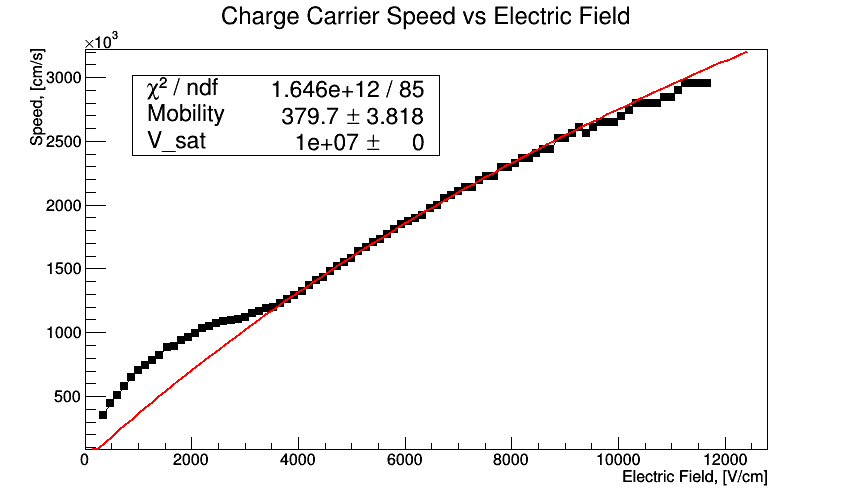
\includegraphics[width=14cm]{pics/top_velocity}
    \caption{The average hole drift velocity for p-type sensor from Particulars.}
    \label{fig:top_velocity}
\end{figure}

The average hole drift velocity through the sensor is given by $v_h = \frac{W}{t_{transit}}$, where $t_{transit}$ is the duration of the signal, $W$ is the thickness of the sensor. For the sample sensor from Particulars the average hole drift velocity is shown in Figure~\ref{fig:top_velocity}. The fit function is given by (\ref{eq:top_velocity_fit}), according to the (\ref{eq:top_velocity}), where $v_{sat}$ is the holes saturation velocity, $\mu_0$ is the low-field mobility, E is the electric field. The fit results in a value of $379.7 \frac{cm^2}{V s}$, with assumption of detector thickness 300 $\mu m$ and saturation velocity in silicon of $v_{sat}=1 \times 10^7 \frac{cm}{s}$.
\begin{equation}
    \centering
    f(E) = \frac{p_0 E}{1+\frac{p_0 E}{v_{sat}}}.
    \label{eq:top_velocity_fit}
\end{equation}
\begin{equation}
    \centering
    v_h(E) = \frac{\mu_0 E}{1+\frac{\mu_0 E}{v_{sat}}}.
    \label{eq:top_velocity}
\end{equation}

\textbf{Realization}

\indent Top TCT Mobility search is realized in the \lstinline$ModuleTopMobility$ class inherited from the \lstinline$TCTModule$ class. The \lstinline$CheckModuleData()$ class method checks that voltage scan contains at least 7 scan points to be sure that velocity dependency vs. voltage can be fitted. The \lstinline$Analysis()$ class method performs velocity dependency building and fitting.

\subsection{Edge TCT}\label{modules:edge}
\subsubsection{Focus Search}\label{modules:edge:focus}

\textbf{Idea}

To find the focus with Edge TCT the same approach is used as for the Top TCT measurements. Instead of scanning and passing the strips, scan is done along the entire detector thickness. The charge profile falling and rising edge are fitted, as it is shown in Figure~\ref{fig:edge_focus}(a). Red arrow shows the direction of the scan. FWHM values are taken from the fits and plotted for different optical distances, then fitted as it shown in Figure~\ref{fig:edge_focus}(b).

\begin{figure}[H]
    \centering
    \subfloat[Schematics]{{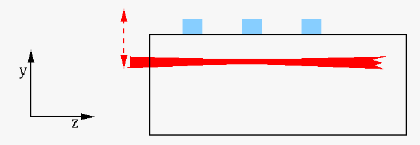
\includegraphics[width=5cm]{pics/edge_focus_0} }}
    \qquad
    \subfloat[FWHM as a function of optical distance, Edge TCT.]{{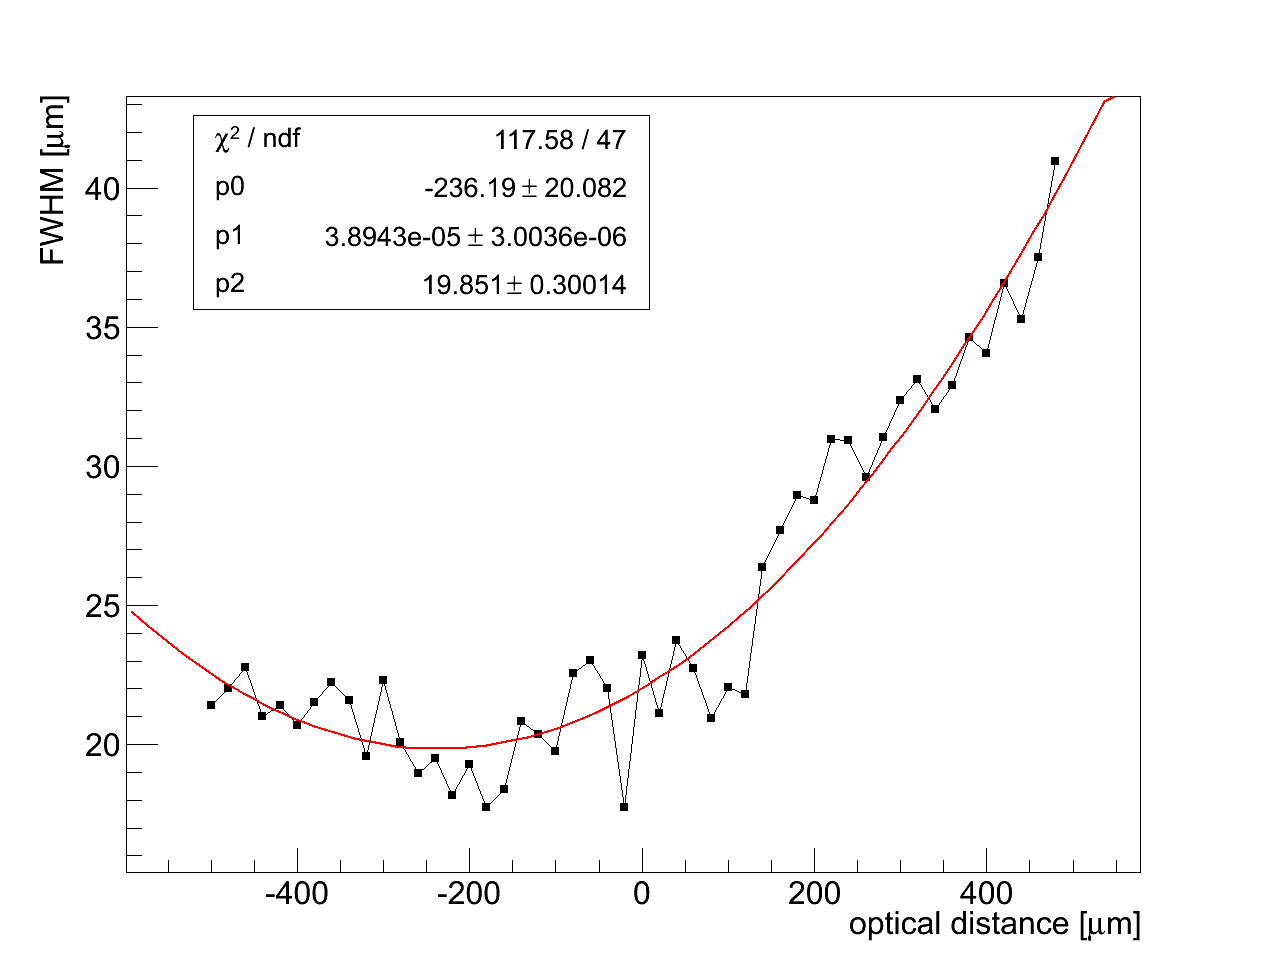
\includegraphics[width=8cm]{pics/edge_focus_1} }}
    \caption{Edge TCT laser beam focusing.}
    \label{fig:edge_focus}
\end{figure}

\textbf{Realization}

\indent Edge TCT Focus Search is realized in the \lstinline$ModuleEdgeFocus$ class inherited from the \lstinline$TCTModule$ class. The \lstinline$CheckModuleData()$ class method checks that scanning axis contains more than 10 scan points to be sure that charge profiles can be fitted. The \lstinline$Analysis()$ class method performs charge profiles building and fitting.

\subsubsection{Depletion Voltage}\label{modules:edge:depl}

\textbf{Idea}

The charge profiles for different bias voltages in arbitrary units are shown in Figure~\ref{fig:edge_charge_profiles}. When the detector is not fully depleted the signal near the bottom of the detector still can be observed due to the different doping concentrations in the n and n+ layers.
\begin{figure}[H]
    \centering
    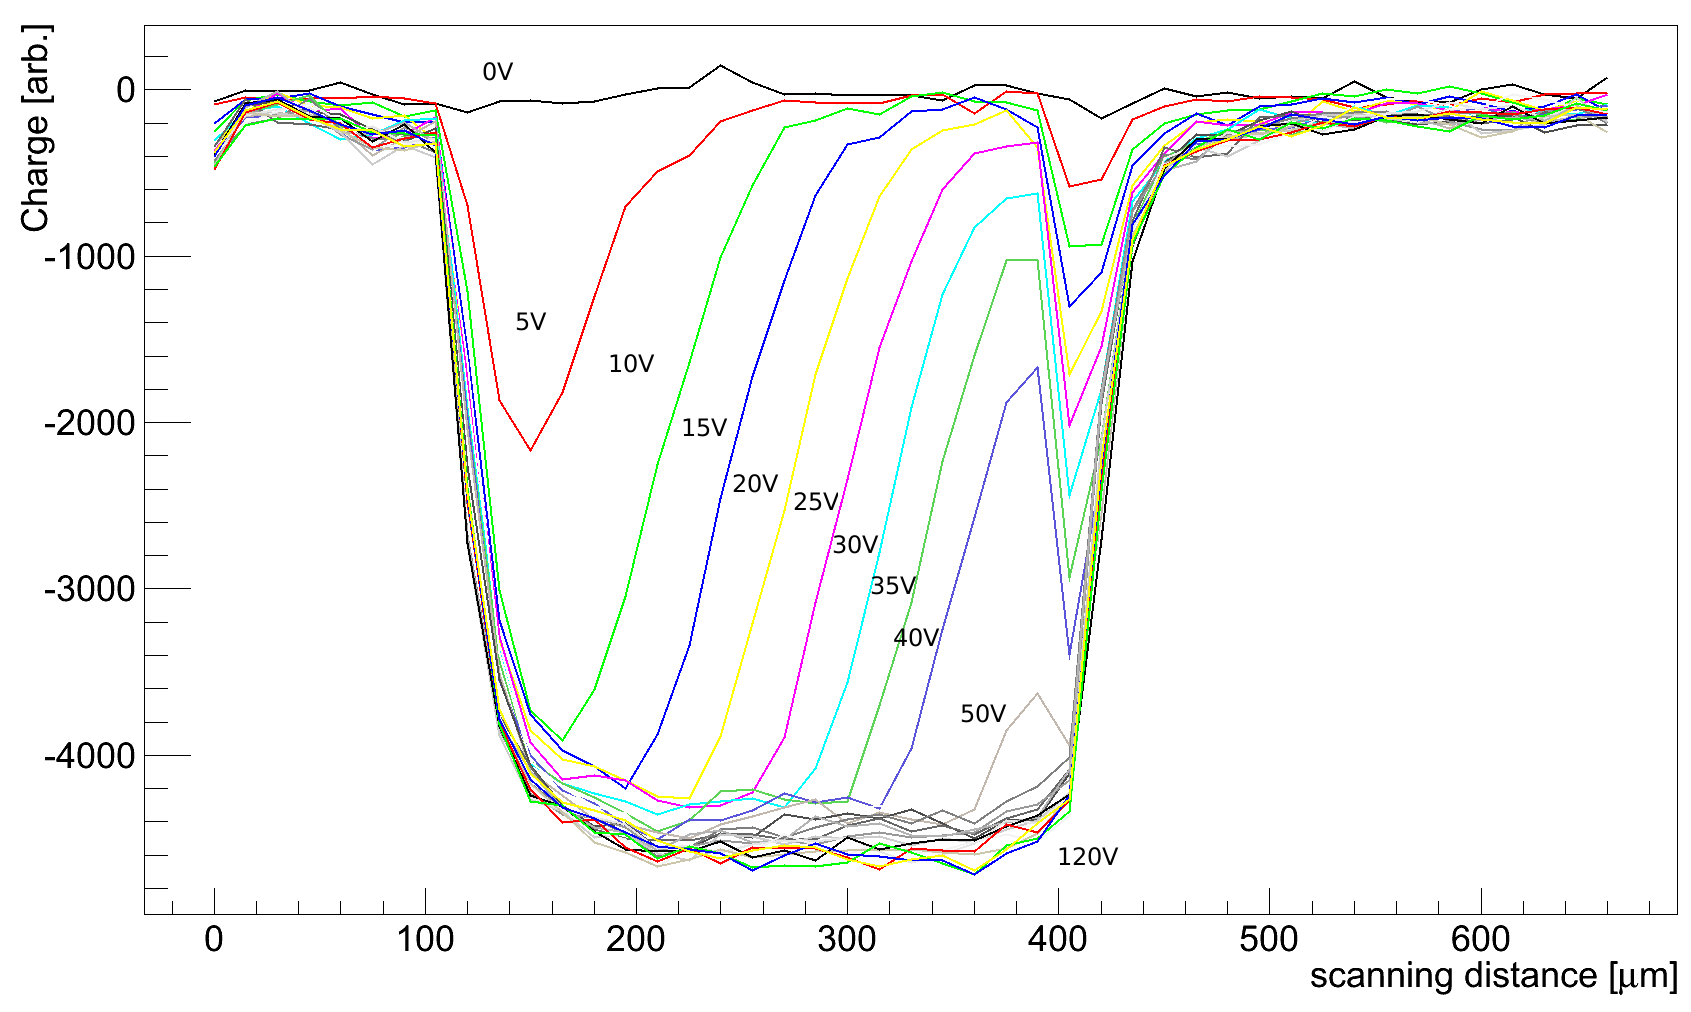
\includegraphics[width=12cm]{pics/edge_charge_profiles}
    \caption{Charge profiles for different voltages, Edge TCT.}
    \label{fig:edge_charge_profiles}
\end{figure}

\begin{figure}[H]
    \centering
    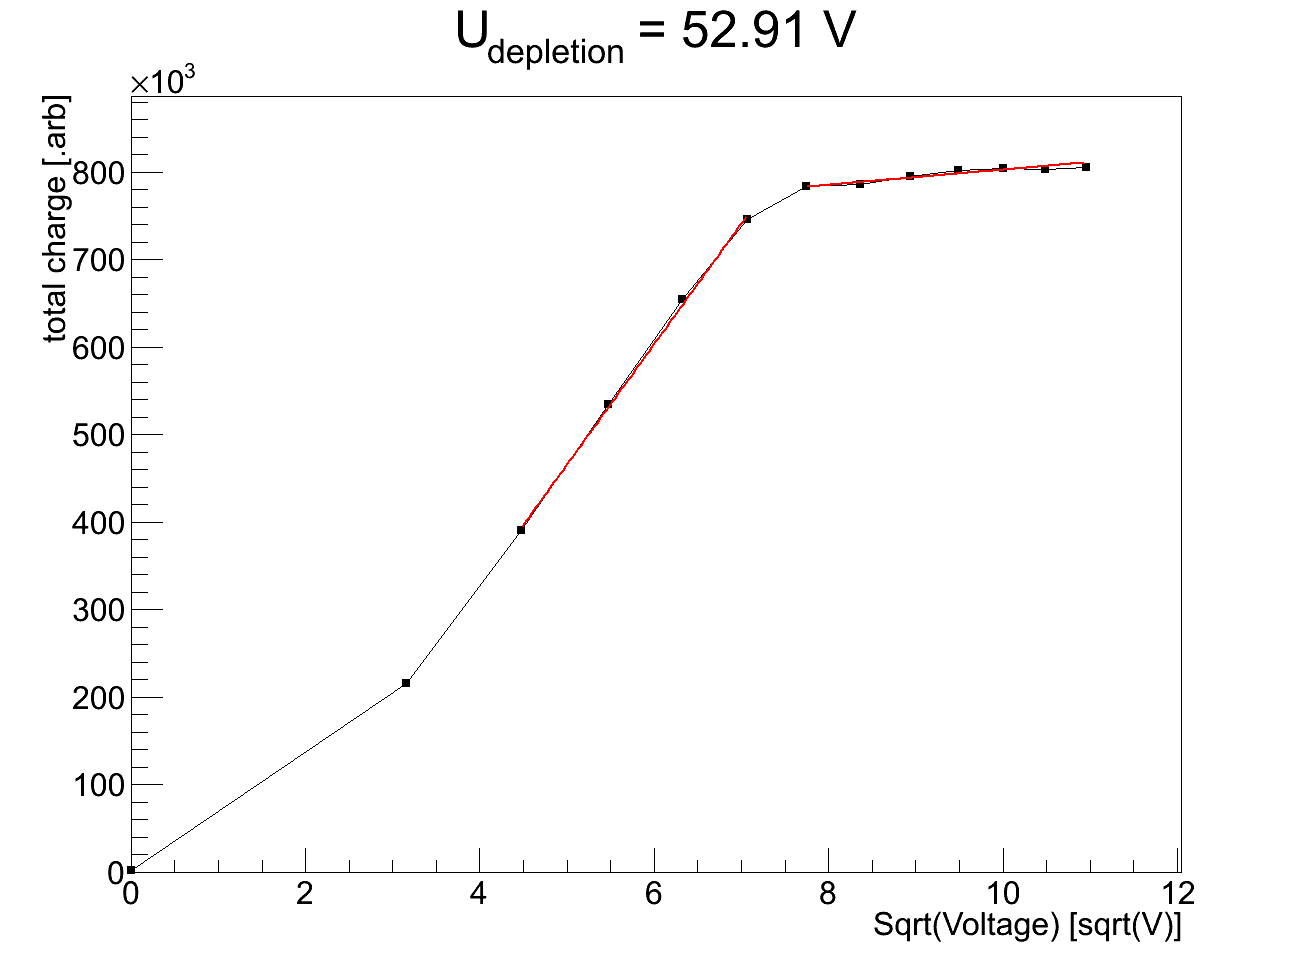
\includegraphics[width=12cm]{pics/edge_depletion}
    \caption{Depletion voltage of the CE2339 sample sensor.}
    \label{fig:edge_depletion}
\end{figure}

Depletion voltage was found using the same method, as it was used for the Top TCT measurements, see Section~\ref{modules:top:depl}, but the charge is also integrated through all the detector thickness. As it shown in Figure~\ref{fig:edge_depletion}, obtained value is 52.91 V and is consistent with the value of 49 V measured using the probe method.

\textbf{Realization}

\indent Edge TCT Depletion Voltage search is realized in the \lstinline$ModuleEdgeDepletion$ class inherited from the \lstinline$TCTModule$ class. The \lstinline$CheckModuleData()$ class method checks that scanning axis contains more than 10 scan points and voltage scan contains at least 7 scan points to be sure that charge dependency vs. voltage can be fitted. The \lstinline$Analysis()$ class method performs charge dependency building and fitting.

\subsubsection{Electric Field Profiles}\label{modules:edge:profiles}

\textbf{Idea}

The induced current in the detector can be expressed by (\ref{eq:edge_current}), where $e_0$ is the elementary charge, $N_{e,h}$ is the number of created e-h pairs near the strip, A is the amplifier amplification, $\tau _{eff,e,h}$ is the effective trapping time, $v_{e,h}$ is the drift velocity and $E_\omega$ is the weighting field. For simple pad detectors term $\overrightarrow{v}_{e,h}(t)\cdot\overrightarrow{E}_{\omega}$ is simply $\frac{v_{e,h}}{W}$, where W is the detector thickness.
\begin{equation}
    \centering
    I_{e,h}(t) = Ae_0N_{e,h}\exp(-\frac{t}{\tau _{eff,e,h}})\overrightarrow{v}_{e,h}(t)\cdot\overrightarrow{E}_{\omega}.
    \label{eq:edge_current}
\end{equation}

According to the Ref. \cite{bib:si_study_edge}, Prompt Current Method is used to obtain the electric field profiles. The measured current amplitude immediately after charge carrier generation ($\exp(-\frac{t}{\tau _{eff,e,h}})\approx1$) can be expressed as:

\begin{equation}
    \centering
    I(y,t\sim0) = Ae_0N_{e,h}\frac{v_e(y)+v_h(y)}{W} = Ae_0N_{e,h}\frac{\mu _e(y)+\mu _h(y)}{W}E(y).
    \label{eq:edge_current_1}
\end{equation}

From this point there could be two ways: one way to extract the electric field profiles is to use the estimation of the charge carriers number from the laser power, measured using the photodetector. But the problem is that one need precise values of the amplification, $N_{e,h}$ - which is difficult to estimate due to the loses in the optical system, in the silicon, etc. The second way is to use formula (\ref{eq:edge_vbias}) as the constraint and to solve numerically the equation (\ref{eq:edge_current_1}). That was done using the bisection method\cite{bib:bisec}. 

\begin{equation}
    \centering
    V_{bias} = \int\limits_0^W E(y) dy.
    \label{eq:edge_vbias}
\end{equation}

\noindent As the result the electric field profiles were extracted and are presented In Figure~\ref{fig:edge_field_profiles}. 

\begin{figure}[h]
    \centering
    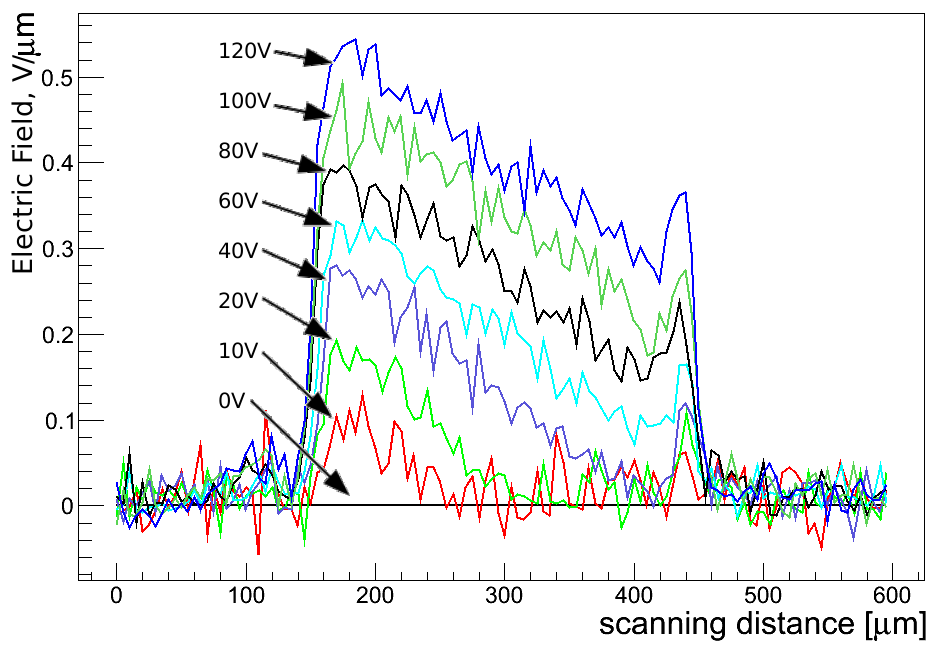
\includegraphics[width=12cm]{pics/edge_field}
    \caption{Field profiles for different voltages, Edge TCT.}
    \label{fig:edge_field_profiles}
\end{figure}

Also the velocity profiles could be extracted using equation (\ref{eq:edge_velocity}), where $v_{sat}$ is the holes saturation velocity, $\mu_0$ is the low-field mobility, E is the electric field.

\begin{equation}
    \centering
    v_h(E) = \frac{\mu_0 E}{1+\frac{\mu_0 E}{v_{sat}}}.
    \label{eq:edge_velocity}
\end{equation}

\textbf{Realization}

\indent Edge TCT Edge Field Profiles search is realized in the \lstinline$ModuleEdgeField$ class inherited from the \lstinline$TCTModule$ class. The \lstinline$CheckModuleData()$ class method checks that scanning axis contains more than 10 scan points to be sure that charge profiles can be fitted. The \lstinline$Analysis()$ class method performs charge profiles building, numerical calculations and output. Also field profiles module contains additionally re-implemented functions and described more advanced in Section~\ref{tutorial_impl}.

\section{Tutorial on TCTModule Implementation}\label{tutorial_impl}

This section is a step by step tutorial on module implementation using \lstinline$ModuleEdgeField$ class (See Section~\ref{modules:edge:profiles}) as the example. 
\\ New module creation consists of several steps:
\begin{enumerate}
\item Module implementation and placement to the \textbf{modules} directory.
\\ Field profiles module was selected due to the presence of several features such as the \lstinline$_EV_Time$ parameter which is used for averaging of the signal during the first moments of evolution - typically less than $1ns$. This parameter is included in the header file, which contains variable definition and set/get methods:
\begin{lstlisting}
public:
		...
        void SetEV_Time(float value) { _EV_Time = value; }
        float GetEV_Time() { return _EV_Time; }
private:
		...
        float _EV_Time;
\end{lstlisting}
As parameter has to be displayed in the GUI, additional methods has to be re-implemented according to Section~\ref{review:tct_module}:
\begin{lstlisting}
public:
	...
#ifdef USE_GUI
        void PrintConfig(std::ofstream &conf_file);
        void AddParameters(QVBoxLayout* layout);
        void FillParameters() { ev_time->setValue(GetEV_Time()); }
        void ToVariables() { SetEV_Time(ev_time->value()); }
        QDoubleSpinBox* ev_time;
#endif
\end{lstlisting}
\lstinline$QDoubleSpinBox* ev_time$ is a graphical widget responsible for parameter input. \lstinline$FillParameters$ and \lstinline$ToVariable$ manipulate with this widget values.
\\ \lstinline$PrintConfig$ is responsible for saving the configuration file with brief explanation of it's meaning:
\begin{lstlisting}
void ModuleEdgeField::PrintConfig(std::ofstream &conf_file) {
    conf_file<<"\n#Averaging the current for electric field profile from F_TLow to F_TLow+EV_Time";
    conf_file<<"\nEV_Time\t=\t"<<GetEV_Time();
}
\end{lstlisting}
\lstinline$AddParameters(QVBoxLayout* layout)$ is used to set the layout of the interface:
\begin{lstlisting}
void ModuleEdgeField::AddParameters(QVBoxLayout *layout) {
    QHBoxLayout* hlayout = new QHBoxLayout;
    hlayout->addStretch();
    hlayout->addWidget(new QLabel("Integration time"));
    ev_time = new QDoubleSpinBox();
    ev_time->setMinimum(0);
    ev_time->setMaximum(1000);
    ev_time->setSingleStep(0.01);
    ev_time->setDecimals(4);
    hlayout->addWidget(ev_time);
    hlayout->addWidget(new QLabel("ns"));
    layout->addLayout(hlayout);
}
\end{lstlisting}
The desired parameter input is shown in Figure~\ref{fig:ev_time}. Horizontal Box Layout used to place the labels and a spin box. 
\begin{figure}[h]
    \centering
    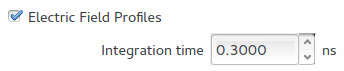
\includegraphics[width=7cm]{pics/ev_time}
    \caption{EV\_Time parameter input.}
    \label{fig:ev_time}
\end{figure}
The \lstinline$CheckModuleData()$ method is easily understandable and will be skipped in this tutorial. The \lstinline$Analysis()$ method is deeply commented, see \textbf{./src/modules/ModuleEdgeField.cc} file.
\item Registering module in the \textbf{tct\_config.cc} source file.
\\ Following discussion is on the \textbf{tct\_config.cc} file. Module has to be included at the beginning of the file:
\begin{lstlisting}
#include "modules/ModuleEdgeField.h"
\end{lstlisting}
When parsing the config file, line to register the module has to be added:
\begin{lstlisting}
if(i.first == "EdgeVelocityProfile")		RegisterModule(new ModuleEdgeField(this,"EdgeVelocityProfile",_Edge, "Electric Field Profiles"), static_cast<bool>(atoi((i.second).c_str())));
\end{lstlisting}
Also EV\_Time parameter has to be set. It has to be added in the second \lstinline$for$ loop, to avoid setting parameter for the non-registered module.
\begin{lstlisting}
if(i.first == "EV_Time")                    ((ModuleEdgeField*)GetModule("EdgeVelocityProfile")) -> SetEV_Time(atof((i.second).c_str()));
\end{lstlisting}
\item Manual adding of the enabling string to the configuration *.txt file.
\\ Has to be done in any configuration file, because module will be registered only if the following line will be present
\begin{lstlisting}
EdgeVelocityProfile = 0
\end{lstlisting}
Parameter EV\_Time does not have to be added, default value $0.3 ns$ will be assigned by default.
\item Running CMake inside the \textbf{build} directory to add module to the build list. Follow building tutorial in Section~\ref{usage:installation}.
\item Code recompilation. Make sure, that needed module was compiled, see Figure~\ref{fig:compiling}.
\begin{figure}[H]
    \centering
    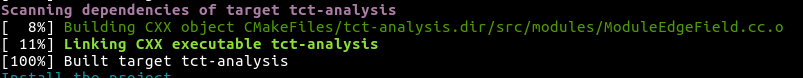
\includegraphics[width=13cm]{pics/compiling}
    \caption{Compilation of new module.}
    \label{fig:compiling}
\end{figure}
\end{enumerate}

\section{Conclusion}

To conclude I would like to express my highest gratitude to Hendrik Jansen(CMS, DESY) for proposing the idea of this framework and sharing of his experience in Transient Current Technique. Also I would like to express my gratitude to ATLAS group(LPNHE, Paris) in the face of Giovanni Calderini, Marco Bomben and Giovanni Marchiori for working with me on establishing TCT test bench at LPNHE and giving an opportunity to continue working on the framework.

In case of additional questions or ideas on improving the documentation (also the framework), please contact me \href{mailto:mykyta.haranko@gmail.com}{mykyta.haranko@gmail.com}
\clearpage 
\appendix
\section{Sample configuration file}\label{App:conf}

Here sample TCT-Analysis configuration file is presented. Follow the comments to understand logic.
\begin{lstlisting}[
    basicstyle=\tiny, %or \small or \footnotesize etc.
]
#comments have to start with a
#put group key words in []
#always specify ID, TAB, "=", TAB, value

[General]
ProjectFolder	=	./
DataFolder	=	../testdata/lpnhe
Outfolder	=	../results/

#Set acq mode.
# 0 - taking the sets of single measurements (*.txt or *.raw files by oscilloscope). Settings are in [Analysis]
# 1 - taking the data from *.tct file produced by DAQ software. Settings are in [Scanning]
Mode	=	1

[Analysis]
MaxAcqs	=	100
Noise_Cut	=	0.005
NoiseEnd_Cut	=	0.005
S2n_Cut	=	3
S2n_Ref	=	2
AmplNegLate_Cut	=	-0.02
AmplPosLate_Cut	=	0.015
AmplNegEarly_Cut	=	-0.02
AmplPosEarly_Cut	=	0.02
DoSmearing	=	0
AddNoise	=	0
AddJitter	=	0
SaveToFile	=	1
SaveSingles	=	1
PrintEvent	=	4294967295
LeCroyRAW	=	0

[Scanning]
#Channels of oscilloscope connected to detector, photodiode, trigger. 
#Put numbers 1,2,3,4 - corresponding to channels, no such device connected put 0.
CH_Detector	=	1
#Turning on of the Photodiode channel also adds normalisation to all scans
CH_Photodiode	=	0
CH_Trigger	=	0
#Set optical Axis. 1-x,2-y,3-z
Optical_Axis	=	3
#Set scanning Axis. 1-x,2-y,3-z
Scanning_Axis	=	1
#Set voltage source number (1 or 2)
Voltage_Source	=	1
#Time between stage movements in seconds.
Movements_dt	=	1
#Set the integration time in ns to correct the bias line. 
#Program averages the signal in range (0,value) and then shifts the signal by the mean value.
CorrectBias	=	5
#Perform next operations. Analysis will start only if all needed data is present:
# 0-top,1-edge,2-bottom
TCT_Mode	=	0

#Scanning over optical and perpendiculr to strip axes 
#(or along the detector depth in case of Edge TCT), fitting the best position.
Focus_Search	=	0
#Depletion Voltage
EdgeDepletionVoltage	=	1
#Electric Field Profiles
EdgeVelocityProfile	=	1
#Averaging the current for electric field profile from F_TLow to F_TLow+EV_Time
EV_Time	=	0.3
#Depletion Voltage
TopDepletionVoltage	=	0
#Charge Carriers Mobility
TopMobility	=	1

#Integrate sensor signal from TimeSensorLow to TimeSensorHigh - ns
TimeSensorLow	=	10
TimeSensorHigh	=	130
#Integrate photodiode signal from TimeDiodeLow to TimeDiodeHigh - ns
TimeDiodeLow	=	46
TimeDiodeHigh	=	51

#Save charge, normed charge and photodiode charge for each Z, voltage
SaveSeparateCharges	=	1
#Save waveforms for each position and voltage
SaveSeparateWaveforms	=	0

[Parameters]
#low-field mobility for electrons, cm2*V^-1*s^-1
Mu0_Electrons	=	1400
#low-field mobility for holes, cm2*V^-1*s^-1
Mu0_Holes	=	450
#saturation velocity cm/s
SaturationVelocity	=	1e+07
# amplifier amplification
Amplification	=	300
# factor between charge in sensor and photodiode due to light splitting: Nsensor/Ndiode
LightSplitter	=	9.65
# resistance of the sensor and diode output, Ohm
ResistanceSensor	=	50
ResistancePhotoDetector	=	50
# pohotodetector responce for certain wavelength, A/W
ResponcePhotoDetector	=	0.7
# electron-hole pair creation energy, eV
EnergyPair	=	3.61

[Sensor]
SampleCard	=	../testsensor/SC_M2015.txt
\end{lstlisting}

\clearpage

\begin{thebibliography}{99}
\begin{sloppypar}
\bibitem{bib:haranko_desy} http://www.desy.de/f/students/2015/reports/MykytaHaranko.pdf
\bibitem{bib:focus} http://particulars.si/downloads/ParticularsProcedures-FocusFind.pdf
\bibitem{bib:opt_si} Green MA, Keevers MJ. Optical properties of intrinsic silicon at 300 K. Progress in Photovoltaics: Research and Applications. 1995 ;3:189 - 192.
\bibitem{bib:ce2339} Jiaguo Zhang DESY-THESIS-2013-018
\bibitem{bib:si_study_edge} G.Kramberger et al, IEEE Transactions on Nuclear Science, vol. 57, no. 4, August 2010.
\bibitem{bib:bisec} https://en.wikipedia.org/wiki/Bisection\_method
\end{sloppypar}
\end{thebibliography}

\end{document}
